\documentclass[a4j,dvipdfmx,autodetect-engine]{jsarticle}
\usepackage[a4paper, total={6.7in, 10.2in}]{geometry}
\usepackage[dvipdfmx]{graphicx}
\usepackage[uplatex,deluxe]{otf}
\usepackage{float}
\usepackage{capt-of}
\usepackage{booktabs}
\usepackage{varwidth}
\usepackage[export]{adjustbox}

% \usepackage{subcaption}
\title{オペアンプ・準備レポート1回目}
\author{TRAN TRUNG DANG KHOA・50011701}

\begin{document}
\maketitle
\begin{enumerate}
    \item TL082のデータシートをインターネット上より調べ、4.1節を完了すること。
    \begin{table}[h]
    \centering
    \caption{TTL082 のデータシート}
    \begin{tabular}{cc}
      \resizebox{0.5\textwidth}{!}{
        \begin{tabular}{l||l} % centered columns (4 columns)
        % \caption{TL082のデータシート} % title of Table
        \hline
        項目 &  値\\ [0.5ex] % inserts table
        %heading
        \hline\hline % inserts single horizontal line
        電源電圧$V_{CC}[V] $ & $\pm 18 $  \\
        同期入力電圧$V_{in}[V] $& $\pm 15 $ \\ 
        異相入力電圧$V_{id}[V]$ & $\pm 30 $ \\
        入力電流$I_B[pA]$ & 50 \\
        利得帯域幅積$GBP[MHz]$& min 2.5, typ 4 \\
        出力電圧振幅$V_O[V]$& $\pm 13.5$\\
        入力抵抗$R_{in}$[$\Omega$]& $10^{12}$ \\
        $入力オフセット電圧V_{OS}[V]$& typ 3, max 10 \\ [1ex]
        \hline %inserts single line
        \end{tabular}%
      }
      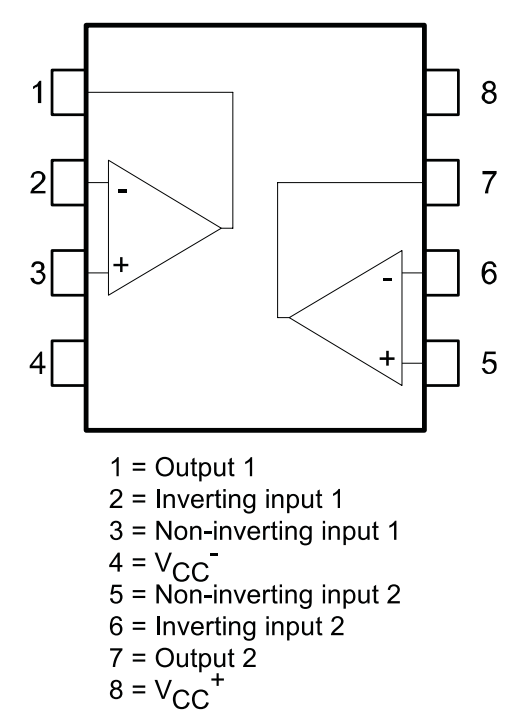
\includegraphics[scale=0.25, valign=m]{tl082-pin.png}
    \end{tabular}
    \label{tab:data_and_fig}
  \end{table}


    \item オペアンプの「入力インピーダンス」の意味、発生理由について調べること。\\
    \quad 入力インピーダンスは動作状態で入力側から見るインピーダンスである。オペアンプでは入力インピーダンスが高いほうが良い。理由としては入力接続先に影響を与えないのである。例えば入力インピーダンスが低いだとすると、オペアンプ内部に電流が流れ込み、入力電圧が降下してしまう。それで、影響を与えていると言える。
    
    
    \item オペアンプの「入力オフセット電圧」の意味、発生理由について調べること。\\
    \quad 出力インピーダンスは動作状態で出力側から見るインピーダンスである。入力インピーダンスと違って、大きくすると、出力電圧が下がってしまうので、低い出力インピーダンスを設計する。
    \item 実験項目4.4.2シュミット回路について、式(1)を導出する。また、実際に実験で使用する抵抗の値を設定すること。\\
    \begin{figure}[H]
        \centering
        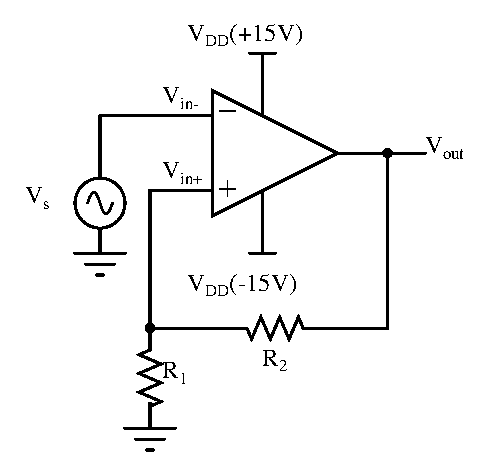
\includegraphics[scale = 0.65]{schmitt.eps}
        \caption{シュミット回路}
        \label{fig:my_label}
    \end{figure}
    図1から見ると$V_{R_1}$が分圧法則を用いて、以下の公式で計算できる。
    \begin{eqnarray}
        V_{R_1} = \frac{R_1}{R_1 + R_2} V_{out} 
    \end{eqnarray}
    シュミット回路はコンパレータ回路の原理と同じだが、GNDと比較する代わりに閾値電圧$V_{R_1}$と比較する。入力信号は反転端子にかけるので閾値電圧を超えると反転する。\\
    実験の設計で仮に$V_{DD} = \pm 15[V], V_{th} = \pm 9.5[V], V_{s} = 10cos(2000\pi t)$ とすると、式(1)によって$R_1とR_2の比例関係は下記に計算できる$
    \begin{eqnarray}
        \frac{R_1}{R_2} = \frac{V_{out}}{V_{R_1}} - 1 = \frac{5.5}{9.5}
    \end{eqnarray}
    したがって、$R_1 = 5.6k\Omega, R_2 = 10k\Omega$を採用できる。
    \item オペアンプの「利得と位相に関する周波数特性」に関する意味、発生理由について調べること。\\
    \quad オペアンプの「利得と位相に関する周波数特性」は出力信号と入力信号の利得と位相が周波数の変化によってどのように変化するのかを意味しいる。理想と違って実際は周波数が高くなると、利得が低下することと位相が遅れることが生じる。理由としてはオペアンプの内部にコンデンサを有するからである。カットオフ周波数を超えるとオペアンプの利得は-20dB/decに従って低下して、無限大に近づくと0になる。位相の変化は低周波数領域では$0^{\circ}$でほとんど変わらないが、カットオフ周波数における$45^{\circ}$
    になり、周波数が無限大になると、位相が$90^{\circ}$に近づいていく。
\end{enumerate}

\bibliographystyle{jplain}
\begin{thebibliography}{3}
\bibitem{1}
STlife.augmented, TL082データシート. 2016年
\bibitem{2}
高崎和之,
ナツメ社,
"基本からわかる電子回路" p.138.
2009年7月
\bibitem{3}
松澤 昭,
講談社,
"はじめてのアナログ電子回路 基本回" pp.113, 175.
2017年2月

\end{thebibliography}

\end{document}
